\documentclass [letter, 12pt]{article}
\usepackage{a4wide, amsmath, amsfonts, amssymb, geometry, shuffle, mathtools}

\usepackage{bm}
\usepackage{fancyhdr, dsfont}
\usepackage[latin1]{inputenc}
\usepackage[pdftex]{graphicx} % uncomment for latex-use
\usepackage{graphicx}
\usepackage{float}
\usepackage{array}
%\usepackage{breqn}
\usepackage[sc,small]{caption}
\setlength{\captionwidth}{15cm} 
%\setlength{\footnotewidth}{15cm} 
\addtolength{\footnotesep}{1mm}
\usepackage{hyperref}
\hypersetup{
    colorlinks=true,
    linkcolor=black,
    citecolor=black,
    filecolor=black,
    urlcolor=black,
    bookmarksdepth=3,
    bookmarksnumbered
}
\usepackage{color}
\definecolor{dgreen}{rgb}{0,0.70,0.30}
\definecolor{gold}{rgb}{0.85,.66,0}
\definecolor{purple}{rgb}{1.0,0.3,0.6}
\definecolor{mathgreen}{rgb}{0,.5,0}

% Package for the pictures
\usepackage{tikz}
\usetikzlibrary{calc} \usetikzlibrary{patterns} \usetikzlibrary{decorations.pathreplacing} \usetikzlibrary{decorations.markings} \usetikzlibrary{decorations.pathmorphing} \usetikzlibrary{positioning}

%%%%%%%%%%%%%%%%  show equation labels  %%%%%%%%%%%%%%%% 
\usepackage[notcite,notref]{showkeys}

\restylefloat{figure}
\usepackage{epstopdf}

%%%%%%%%


\def\beq{\begin{equation}}
\def\eeq{\end{equation}}
\let\Re\relax
\let\Im\relax
\DeclareMathOperator{\Re}{Re}
\DeclareMathOperator{\Im}{Im}

\newcommand{\co}{\ , \ \ \ \ \ \ }
\newcommand{\dd}{\mathrm{d}}
\newcommand{\te}{\textrm}
\newcommand{\ap}{\alpha'}

\newcommand{\nn}{\nonumber}

% Zahlenmengen
\newcommand{\RR}{\mathbb R}
\newcommand{\CC}{\mathbb C}
\newcommand{\NN}{\mathbb N}
\newcommand{\ZZ}{\mathbb Z}
\newcommand{\QQ}{\mathbb Q}

% mathfrak commands
\newcommand{\efrak}{\mathfrak e}
\newcommand{\ffrak}{\mathfrak f}

%\renewcommand{\theta}{\vartheta}
\newcommand{\mb}[1]{\textcolor{blue}{\bf Marcus: [#1]}\marginpar[\hfill${\bf \Longrightarrow}$]%
                  {${\bf \Longleftarrow}$} }                  
\newcommand{\be}{\begin{equation}}
\newcommand{\ee}{\end{equation}}
\newcommand{\bea}{\begin{eqnarray}}
\newcommand{\eea}{\end{eqnarray}}

% Marcus macros
\newcommand{\tht}{\vartheta}

% Igor's macros

\linespread{1.4}
% Kontrolliert Zeilenabstand
\geometry{right=15mm, bottom=20mm, left=15mm, top=17mm}
% Kontrolliert Abstand des Textes vom Seitenrand
\interfootnotelinepenalty=10000

\title{\vspace{1cm}\textbf{Reducing one-loop correlators to bases of worldsheet functions} \\ \ \\} % Titel - wird in diesem Fall fett gedruckt
\author{\hspace{-0cm}some people\\[5mm]
\hspace{-0cm} $^{a}$
{\it some}\\[-1mm] {\it affiliations} 
}


\begin{document}

\centerline{\Large{Notes on $\det'A$}}
 ~\\
 
 
Consider the $n\times n$ symmetric matrix $A_n$. We rewrite every diagonal element 
0 as the sum of the remaining elements in the row (column). We  
  delete the $n$-th  row and column at first. For the 
  remaining $(n-1)\times (n-1)$ symmetric matrix, we can still let every diagonal element as the sum of the remaining elements in the row (column) by using ${\rm SL}(2)$ gauge to
 send $\sigma_n$ to infinity.   Now we can use the matrix tree theorem \footnote{Note that the matrix tree theorem itself doesn't require the matrix is symmetric.}. We choose to continue to delete the  $1$-th  row and column. Then  the determinant of the remaining 
 $(n-2)\times (n-2)$ symmetric matrix can be written as a sum of all labelled trees made up by $(n-1)$ nodes and $(n-2)$ directed edges.   All  directions  are determined by requiring all flows end at node 1. See figure \ref{fig:universe} as an example of 4pt.
 \begin{figure}[h!]
\centering
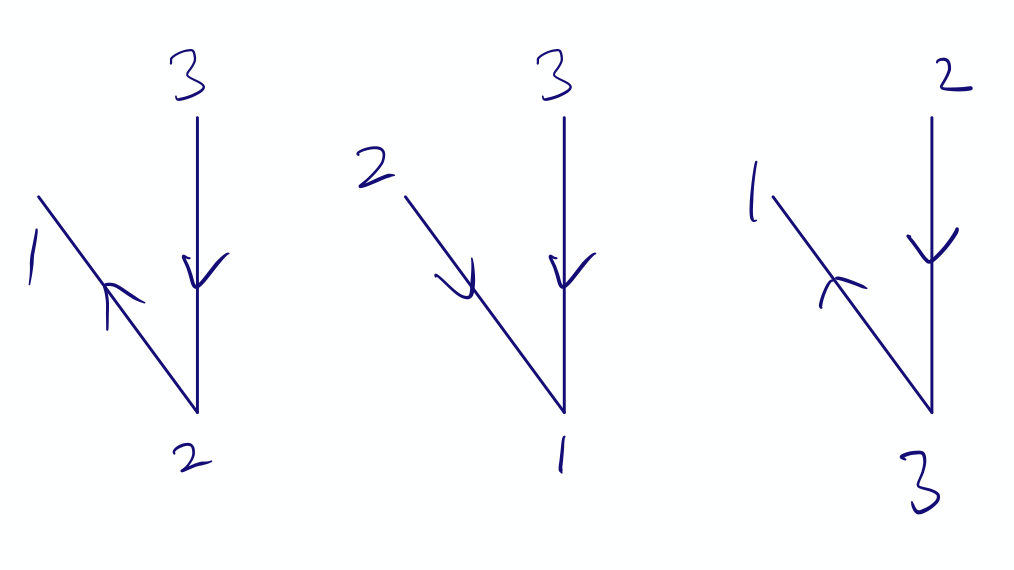
\includegraphics[scale=.5]{4pt.PNG}
\caption{4pt example}
\label{fig:universe}
\end{figure}
 Each directed edge $i\to j$ represents a factor $\frac{s_{ij}}{\sigma_{ij}}$ and each labelled tree denoted as ${\cal T}$ represents a product of $(n-2)$ such factors denoted as $P({\cal T})$.
 
   
 Consider the soft limit of particle $i$, i.e. $s_{ij}\to \tau {\hat s}_{ij}$ with $\tau \to 0$ for any $j\neq i$. Obviously, if the node $i$ is linked by $r$ edges in a labelled tree ${\cal T}$, the corresponding product $P({\cal T})$  will vanish at order ${\cal O}(\tau^r)$.  Thus we only need to consider such labelled trees where the node $i$ is only linked by one edge, i.e. the  node $i$  is on the ends of the tree.  If we remove the node  $i$ and the only edge connecting to it, the remaining part is still a labelled tree of lower points. For any such $(n-2)$-pt labelled tree, we can see the node $i$ can connect to any node the $(n-2)$-pt labelled tree through an edge, resulting in a sum factor $\sum_{j\neq i}\frac{s_{ij}}{\sigma_{ij}}=0$. This explains the Alder zero.   
 
 
\end{document}



\centerline{\Large{JHEP}}

~\\

Recently,  the generalized biadjoint amplitudes for higher $k$ have been proposed and  have been found closely related to tropical Grassmannians, cluster algebras and so on.  Following the paper of 1907.01053,  this paper provides a more systematic way to  utilize the cluster algebras and more results of tropical Grassmannians are got.  For $k=4,n=8$,  the corresponding cluster algebra is infinite type and this paper shows how to use the limits of mutation sequences in detail to get the last 4 rays of the corresponding tropical Grassmannians. 


There is a small typo "Grassmanians" in the abstract. Besides,
 I think the new version of this paper has been well organized. 
It is an important contribution to the literature on scattering equations and thus I recommend it for publication in JHEP.



the scattering equations on X(2, n) have been generalized to higher dimensional projective spaces by Cachazo and collaborators. In this construc- tion, the space X(2, n) is replaced by the space X(k, n). The paper continues the study of the solutions of these generalized scattering equations for k > 2.
The solutions include both regular and singular solutions. In the previous paper (ref [5]) regular solutions were studied, and it was shown that they can not account for all solutions. In this paper the authors have initiated the study of singular solutions, and found them for all cases with n < 9 except for X(4, 8). They also make a proposal for all configurations that can support singular solutions.
The observation about the relation between the number of solutions and the number of representations of uniform matroids over finite fields is espe- cially very interesting.







\centerline{\Large{Notes on double pole 3pt integral}}

~\\

Consider length-3 subcycle integral,
\begin{equation}
Z_{\rm DP3}=\int dz_2 dz_3 \Omega(z_{12},\beta,\tau)\Omega(z_{23},\xi,\tau)\Omega(z_{31},\gamma,\tau).
\end{equation}
We use the Fay identity to reduce the length-3 subcycle as  length-2 ones,
\be\label{fjadf}
 \Omega(z_{12},\beta,\tau)\Omega(z_{23},\xi,\tau)\Omega(z_{31},\gamma,\tau)=\Big(
\Omega(z_{12},\beta+\gamma,\tau)\Omega(z_{32},\gamma,\tau)- \Omega(z_{31},\beta+\gamma,\tau)\Omega(z_{32},-\beta,\tau)
 \Big)\Omega(z_{23},\xi,\tau)
\ee
where  we have used $ \Omega(-z,-\eta,\tau)= -\Omega(z,\eta,\tau)$ ({\color{blue}Is this identity true?{\footnote{What really puzzles me is $ \partial_{z_2} \Omega(z_{23},\xi,\tau) $. According to differential link rules, it seems we have 
$\partial_{z_2} \Omega(z_{23},\xi,\tau) =-\partial_{z_3} \Omega(z_{23},\xi,\tau) $.   However, we can write $\Omega(z_{23},\xi,\tau) $ as $-\Omega(z_{32},-\xi,\tau) $ at first, then $\partial_{z_2}\Big(-\Omega(z_{32},-\xi,\tau)\Big)=  -\partial_{z_2}\Omega(z_{32},-\xi,\tau)=  \partial_{z_3}\Omega(z_{32},-\xi,\tau)$, which leads to $\partial_{z_2} \Omega(z_{23},\xi,\tau) =\partial_{z_3}\Omega(z_{32},-\xi,\tau)$. Sorry for my shortness of related background knowledge. 
}}}). In the first term on the RHS,  there is a length-2 subcycle $ \Omega(z_{32},\cdots) \Omega(z_{23},\cdots)$ and a branch $\Omega(z_{12},\cdots)$ planted on it through $z_2$. 
Inspired by the experience in dealing with tree-level analogs,  we try to use the vanishing of the total derivative of  $z_3$ to break the subcycle $ \Omega(z_{32},\cdots) \Omega(z_{23},\cdots)$.  Following the steps in the Oliver's draft on double pole 2pt integral,    first we  rewrite the subcycle via (2.21) in the Oliver's proceedings note
\be\label{afipo}
\Omega(z_{23},\xi,\tau)\Omega(z_{32},\gamma,\tau)
=\partial_3 \Omega(z_{23},\xi-\gamma,\tau)+\Omega(z_{23},\xi-\gamma,\tau)(\hat{g}^{(1)}(\gamma,\tau)-\hat{g}^{(1)}(\xi,\tau)).
\ee 
({\color{blue} It seems this equality holds locally no matter what the remaining is in the integrand, for example, $\Omega(z_{12},\beta+\gamma,\tau)$ here. Is it true?}) Then,  eliminate $\partial_3 \Omega(z_{23},\cdots)$ via (2.12) in the Oliver's proceedings note,
\be
\partial_3 \Omega(z_{23},\xi-\gamma,\tau)=\partial_\xi \Omega(z_{23},\xi-\gamma,\tau)+\Big(\hat{g}^{(1)}(\xi-\gamma,\tau)-f^{(1)}(z_{23},\tau)\Big)\Omega(z_{23},\xi-\gamma,\tau),
\ee 
with $f^{(1)}(z_{23},\tau)$ to be further dealt with ({\color{blue} Again, does this equality hold locally?}). The above two equations have no analogs in the tree-level cases. 

Now, we consider integration-by-parts to relate  $\partial_3 \Omega(z_{23},\xi-\gamma,\tau) $ and   $f^{(1)}(z_{23},\tau)\Omega(z_{23},\xi-\gamma,\tau)$,
\be
\partial_3 \Omega(z_{23},\xi-\gamma,\tau) \Omega(z_{12},\beta+\gamma,\tau) {\rm KN} \overset{\rm IBP}{\cong} \Big( s_{13}f^{(1)}(z_{13},\tau)+s_{23}f^{(1)}(z_{23},\tau) \Big)\Omega(z_{23},\xi-\gamma,\tau) \Omega(z_{12},\beta+\gamma,\tau)  {\rm KN}\,,
\ee
where $\Omega(z_{12},\beta+\gamma,\tau) $ doesn't contain $z_3$ and hence we only need to consider the derivative of KN.  Different from the 2pt case, there are two terms appearing,  with the first one $s_{13}f^{(1)}(z_{13},\tau)$ very annoying. 
According to the above two simultaneous equations, we can get 
\bea
\partial_3 \Omega(z_{23},\xi-\gamma,\tau)&{\cong}&
\Big[\frac{s_{23}}{1+s_{23}} \Big(\partial_\xi +  \hat{g}^{(1)}(\xi-\gamma,\tau)\Big)+\frac{s_{13}}{1+s_{23}} f^{(1)}(z_{13},\tau) \Big] \Omega(z_{23},\xi-\gamma,\tau) \,,
\nonumber
\\
s_{23}f^{(1)}(z_{23},\tau)  \Omega(z_{23},\xi-\gamma,\tau)&{\cong}&
\Big[\frac{1}{1+s_{23}} \Big(\partial_\xi +  \hat{g}^{(1)}(\xi-\gamma,\tau)\Big)-\frac{s_{13}}{1+s_{23}} f^{(1)}(z_{13},\tau) \Big] \Omega(z_{23},\xi-\gamma,\tau) \,.
\nonumber
\\
\eea
With this solution, we can only write the first term on the RHS of \eqref{fjadf} as 
\bea\label{jashdlfi}
&&
\Omega(z_{12},\beta+\gamma,\tau)\Omega(z_{32},\gamma,\tau)\Omega(z_{23},\xi,\tau)
\\
\overset{\rm IBP}{\cong}&&\Big[\frac{s_{23}}{1+s_{23}} \Big(\partial_\xi +  \hat{g}^{(1)}(\xi-\gamma,\tau)\Big)+\frac{s_{13}}{1+s_{23}} f^{(1)}(z_{13},\tau)  +\Big(\hat{g}^{(1)}(\gamma,\tau)-\hat{g}^{(1)}(\xi,\tau)\Big) \Big]
\nonumber
\\
&&\times\Omega(z_{23},\xi-\gamma,\tau) \Omega(z_{12},\beta+\gamma,\tau) \,,
\nonumber
\eea
with a new length-3 subcycle $f^{(1)}(z_{13},\tau) \Omega(z_{12},\beta+\gamma,\tau) \Omega(z_{23},\xi-\gamma,\tau) $ to be further dealt with. 



Similarly,  for the second  term on the RHS of \eqref{fjadf},  we have 
\bea\label{jashdlfi2}
&&
-\Omega(z_{31},\beta+\gamma,\tau)\Omega(z_{23},\xi,\tau)\Omega(z_{32},-\beta,\tau)
\\
\overset{\rm IBP}{\cong}&&\Big[\frac{s_{23}}{1+s_{23}} \Big(\partial_\xi +\hat{g}^{(1)}(-\xi-\beta,\tau)\Big)+\frac{s_{12}}{1+s_{23}} f^{(1)}(z_{12},\tau)  +(\hat{g}^{(1)}(-\beta,\tau)-\hat{g}^{(1)}(\xi,\tau)) \Big]
\nonumber
\\
&&\times\Omega(z_{31},\beta+\gamma,\tau) \Omega(z_{23},\xi+\beta,\tau)\,,
\nonumber
\eea
with $f^{(1)}(z_{12},\tau) \Omega(z_{31},\beta+\gamma,\tau) \Omega(z_{23},\xi+\beta,\tau) $ to be further dealt with.  


I have tried many methods  to eliminate the new kind of  length-3 subcycles $f^{(1)}(\cdots)\Omega(\cdots)\Omega(\cdots)$ including transforming them as the form  $\Omega(z_{12},\cdots)\Omega(z_{23},\cdots)\Omega(z_{31},\cdots)$
but all failed. New insights are needed. 


As a desperate try, I 
 made use of the vanishing of the total derivative of other punctures, for example,  $z_2$   for the first  term on the RHS of \eqref{fjadf}.
I rewrote $\Omega(z_{23},\xi,\tau)\Omega(z_{32},\gamma,\tau)$ as $\Omega(z_{32},-\xi,\tau)\Omega(z_{23},-\gamma,\tau)$ and similar to \eqref{afipo}  we had
\be
\Omega(z_{32},-\xi,\tau)\Omega(z_{23},-\gamma,\tau)
=\partial_2 \Omega(z_{32},-\xi+\gamma,\tau)+\Omega(z_{32},-\xi+\gamma,\tau)(\hat{g}^{(1)}(-\gamma,\tau)-\hat{g}^{(1)}(-\xi,\tau)),
\ee 
with
\be
\partial_2 \Omega(z_{32},-\xi+\gamma,\tau)=\partial_\beta \Omega(z_{32},-\xi+\gamma,\tau)+\Big(\hat{g}^{(1)}(-\xi+\gamma,\tau)-f^{(1)}(z_{32},\tau)\Big)\Omega(z_{32},-\xi+\gamma,\tau).
\ee 
The IBP calculation became tougher but I finished it by brute-force,
\bea
\partial_2 \Omega(z_{32},-\xi-\gamma,\tau) \Omega(z_{12},\beta+\gamma,\tau) {\rm KN} &\!\!\!\overset{\rm IBP}{\cong}\!\!\!
& \Big( s_{12}f^{(1)}(z_{12},\tau)+s_{23}f^{(1)}(z_{32},\tau) \Big)\Omega(z_{32},-\xi-\gamma,\tau) \Omega(z_{12},\beta+\gamma,\tau) {\rm KN}
\nonumber
\\
&&- \Omega(z_{32},-\xi-\gamma,\tau) \partial_2 \Omega(z_{12},\beta+\gamma,\tau) {\rm KN} 
 \,,
\eea
with
\be
\partial_2 \Omega(z_{12},\beta+\gamma,\tau)=\partial_\beta \Omega(z_{12},\beta+\gamma,\tau)+\Big(\hat{g}^{(1)}(\beta+\gamma,\tau)-f^{(1)}(z_{12},\tau)\Big)\Omega(z_{12},\beta+\gamma,\tau).
\ee 

According to the above three simultaneous equations, I solved $\partial_2 \Omega(z_{32},-\xi-\gamma,\tau) ,  \partial_2 \Omega(z_{12},\beta+\gamma,\tau)$ and $ f^{(1)}(z_{32},\tau)$ at the price of introducing $ f^{(1)}(z_{12},\tau)$ and finally expressed the  first term on the RHS of \eqref{fjadf} as 
\bea\label{fauisd}
&&
\Omega(z_{12},\beta+\gamma,\tau)\Omega(z_{32},\gamma,\tau)\Omega(z_{23},\xi,\tau)
\\
\overset{\rm IBP}{\cong}&&
\frac{s_{23}}{1+s_{23}} \Big[\Big(\partial_\gamma +  \hat{g}^{(1)}(-\xi-\gamma,\tau)- \hat{g}^{(1)}(-\xi,\tau)\Big)
 \Omega(z_{23},\xi+\gamma,\tau) \Big]\Omega(z_{12},\beta+\gamma,\tau)
 \nonumber
\\
&&-\frac{1}{1+s_{23}} \Big[\Big(\partial_\gamma +  \hat{g}^{(1)}(\beta+\gamma,\tau)+ \hat{g}^{(1)}(-\xi,\tau)\Big)
\Omega(z_{12},\beta+\gamma,\tau) \Big]\Omega(z_{23},\xi+\gamma,\tau)
\nonumber
 \\
&&+\Big[\frac{1+s_{12}}{1+s_{23}} f^{(1)}(z_{12},\tau)  +\hat{g}^{(1)}(\gamma,\tau)  \Big]\Omega(z_{12},\beta+\gamma,\tau) \Omega(z_{23},\xi+\gamma,\tau)\,.
\nonumber
\eea
We can see we have introduced another equality \eqref{fauisd}  in addition to \eqref{jashdlfi}  but another new variable  came out as well. 
There are $f^{(1)}(z_{12},\tau)$ factor in both \eqref{jashdlfi2} and \eqref{fauisd}, but many things are left to be done to eliminate this factor because the two equalities  are not really identities but only hold on the support of IBP.  I will read Oliver's proceedings note more carefully, which mainly focuses on dealing with the subcycles of $f^{(k)}$ factors and check if I can learn some skills to handle the present problems.

\end{document}



\maketitle{}
\vspace{1cm}
\begin{abstract}
We reduce genus-one correlators of bosonic, heterotic and supersymmetric string theories
 to a universal basis of worldsheet functions. This is the one-loop analogue of the research programm
 on string tree-level amplitudes in \cite{Huang:2016tag, Azevedo:2018dgo, He:2018pol, He:2019}.
\end{abstract}


\newpage

\setcounter{tocdepth}{2}
\tableofcontents


\numberwithin{equation}{section}

%%%%%%%%%%%%%%%%%%%%%%%%%%%%%%%%%%%%%%%%%%%%%%%%%%%%%%%
%%%%%%%%%%%%%%%%%%%%%%%%%%%%%%%%%%%%%%%%%%%%%%%%%%%%%%%




\section{Introduction}
%%%%%%%%%%%%%%%%%%%%%%%%%%%%%%%%%%%%%%%%%%%%%%%%%%%%%%%
%%%%%%%%%%%%%%%%%%%%%%%%%%%%%%%%%%%%%%%%%%%%%%%%%%%%%%%


 

%%%%%%%%%%%%%%%%%%%%%%%%%%%%%%%%%%%%%%%%%%%%%%%%%%%%%%%
%%%%%%%%%%%%%%%%%%%%%%%%%%%%%%%%%%%%%%%%%%%%%%%%%%%%%%%
\section{Doubly-periodic functions}
\label{sec:2}
%%%%%%%%%%%%%%%%%%%%%%%%%%%%%%%%%%%%%%%%%%%%%%%%%%%%%%%
%%%%%%%%%%%%%%%%%%%%%%%%%%%%%%%%%%%%%%%%%%%%%%%%%%%%%%%


%%%%%%%%%%%%%%%%%%%%%%%%%%%%%%%%%%%%%%%%%%%%%%%%%%%%%%%
\subsection{Basic definitions}
\label{sec:2.2}
%%%%%%%%%%%%%%%%%%%%%%%%%%%%%%%%%%%%%%%%%%%%%%%%%%%%%%%

All the dependence of genus-one correlators on the punctures will
be deduced from the Kronecker--Eisenstein series
%
\begin{equation}
F(z,\beta,\tau) \equiv \frac{ \theta'(0,\tau) \theta(z+\beta,\tau) }{\theta(z,\tau)  \theta(\beta,\tau)}
\label{1.2}
\end{equation}
%
and its doubly-periodic completion
%
\begin{equation}
\Omega(z,\beta,\tau) \equiv \exp\Big( 
2\pi i \beta \, \frac{ \Im  z}{\Im  \tau} \Big)
\, F(z,\beta,\tau) \ .
\label{1.1}
\end{equation}
%
The non-holomorphic exponential drops out from cyclic products of (\ref{1.1}) which generate elliptic 
functions $V_w(1,2,\ldots,n)$ upon expansion in the formal bookkeeping variable $\beta$,
\begin{align}
&F(z_{12},\beta,\tau) F(z_{23},\beta,\tau) \ldots F(z_{n,1},\beta,\tau) = \Omega(z_{12},\beta,\tau) \Omega(z_{23},\beta,\tau) \ldots \Omega(z_{n,1},\beta,\tau)
\notag \\
%
&= \beta^{-n} \sum_{w=0}^\infty \beta^w V_w(1,2,\ldots,n)  \ . \label{1.1a}
\end{align}
Their definition via (\ref{1.1a}) immediately manifests cyclicity $V_w(1,2,\ldots,n) = V_w(2,\ldots,n,1)$, and
the symmetry property $F(-z,-\beta,\tau) = - F(z,\beta,\tau)$ leads to the $w$-dependent reflection property
\begin{equation}
V_w(n,n{-}1,\ldots,2,1) = (-1)^w V_w(1,2,\ldots,n)
\end{equation}
upon reversal of the cycle $1,2,\ldots,n$. The $V_w$ can be conveniently expressed in terms of the
doubly-periodic coefficients $f^{(0)}=1$ and 
$f^{(1)}(z,\tau) = \partial_z \log \theta(z,\tau) + 2\pi i \frac{ \Im z}{\Im  \tau}, \ldots$ defined by
\begin{equation}
\Omega(z,\beta,\tau) \equiv \sum_{w=0}^{\infty} \beta^{w-1} f^{(w)}(z,\tau)\ ,
\label{1.1b}
\end{equation}
for instance (with cyclic identification $z_{n+1}=z_1$)
\begin{align}
V_0(1,2,\ldots,n) &=1 \ , \ \ \ \ \ \  V_1(1,2,\ldots,n) = \sum_{j=1}^n f^{(1)}(z_{j}{-}z_{j+1},\tau) \label{1.1c} \\
%
V_2(1,2,\ldots,n) &= \sum_{j=1}^n f^{(2)}(z_{j}{-}z_{j+1},\tau)
+\sum_{i=1}^n \sum_{j=i{+}1}^n f^{(1)}(z_{i}{-}z_{i+1},\tau)f^{(1)}(z_{j}{-}z_{j+1},\tau) \ .
\notag
\end{align}
%
Evaluating the $f^{(k)}(z,\tau)$ at the origin reproduces holomorphic Eisenstein series 
\begin{equation}
{\rm G}_k(\tau) \equiv  \sum_{(m,n) \neq (0,0)} \frac{1}{(m\tau + n)^{k}} = - f^{(k)}(0,\tau),\qquad k\geq 4   \ .
\label{1.6}
\end{equation}
%
Note that the $z\rightarrow 0 $ limit of $f^{(2)}(z,\tau)$ is ill-defined. Still, we will later encounter
the non-holomorphic but modular representative of the weight-two Eisenstein series
 \begin{equation}
\hat {\rm G}_2(\tau) \equiv  \lim_{s\rightarrow 0}\sum_{(m,n) \neq (0,0)} \frac{1}{(m\tau + n)^{2} \,|m\tau + n|^s} \equiv  {\rm G}_2(\tau)  - \frac{\pi}{\Im  \tau}\, .
\end{equation}
%
Note that the Weierstrass function can be represented in the following ways
%
\begin{align}
  V_{2}(1,2)= 2 f^{(2)}(z_{1}{-}z_2,\tau) - ( f^{(1)}(z_{1}{-}z_2,\tau))^2
 = -\wp(z_{12},\tau)= \partial^2 \log \theta(z_1{-}z_2,\tau)+{\rm \hat G}_{2}(\tau)\ .
\end{align}
%
A collection of identities among the $f^{(k)}(z,\tau)$ can be found in section 3 of \cite{Broedel:2014vla}.

%%%%%%%%%%%%%%%%%%%%%%%%%%%%%%%%%%%%%%%%%%%%%%%%%%%%%%%
\subsection{$z$-derivatives}
\label{sec:2.0}
%%%%%%%%%%%%%%%%%%%%%%%%%%%%%%%%%%%%%%%%%%%%%%%%%%%%%%%

The derivatives of $f^{(k)}(z,\tau)$ w.r.t.\ the first argument can be rewritten as
%
\begin{align}
\partial_z f^{(1)}(z,\tau) &= 2 f^{(2)}(z,\tau) - \big( f^{(1)}(z,\tau) \big)^2 - {\rm \hat G}_2(\tau) \notag \\
%
\partial_z f^{(2)}(z,\tau) &= 3 f^{(3)}(z,\tau) -  f^{(1)}(z,\tau)   f^{(2)}(z,\tau)  - {\rm \hat G}_2(\tau)  f^{(1)}(z,\tau)  \notag \\
%
\partial_z f^{(3)}(z,\tau) &= 4 f^{(4)}(z,\tau) -  f^{(1)}(z,\tau)   f^{(3)}(z,\tau)  - {\rm \hat G}_2(\tau)  f^{(2)}(z,\tau) - {\rm G}_4(\tau)
 \label{uniform04} \\
 %
\partial_z f^{(4)}(z,\tau) &= 5 f^{(5)}(z,\tau) -  f^{(1)}(z,\tau)   f^{(4)}(z,\tau)  - {\rm \hat G}_2(\tau)  f^{(3)}(z,\tau) - {\rm G}_4(\tau)  f^{(1)}(z,\tau) \notag \\
%
\partial_z f^{(5)}(z,\tau) &=  6 f^{(6)}(z,\tau) -  f^{(1)}(z,\tau)   f^{(5)}(z,\tau)  - {\rm \hat G}_2(\tau)  f^{(4)}(z,\tau) - {\rm G}_4(\tau)  f^{(2)}(z,\tau)- {\rm G}_6(\tau)\ , \notag
\end{align}
%
and more generally
%
\begin{align}
  \partial_{z}f^{(n)}(z,\tau)&=(n{+}1)f^{(n+1)}(z,\tau)-f^{(1)}(z,\tau)f^{(n)}(z,\tau)   \label{uniform00}\\
  %
  & \ \ \ \ -{\rm \hat G}_{2}(\tau)f^{(n-1)}(z,\tau)-\sum_{m=4}^{n+1}{\rm G}_{m}(\tau)f^{(n-m+1)}(z,\tau)\ . \notag
\end{align}
%
This follows from the generating-function identity
%
\begin{align}
  \partial_{z}\Omega(z,\alpha,\tau)-\partial_{\alpha}\Omega(z,\alpha,\tau)=(\hat g^{(1)}(\alpha,\tau)-f^{(1)}(z,\tau))
  \Omega(z,\alpha,\tau)\, ,
  %-\frac{\pi\alpha}{\tau_{2}}\Omega(z,\alpha,\tau)\ .
  \label{eq:134}
\end{align}
%
where
%
\beq
\hat g^{(1)}(\alpha,\tau) = \partial_\alpha \log \theta(\alpha,\tau)  + \frac{ \pi \alpha}{\Im \tau} =  \frac{1}{\alpha} - \alpha \hat {\rm G}_2(\tau)
-\sum_{n=4}^{\infty} \alpha^{n-1} {\rm G}_n(\tau) 
\eeq
%
and 
%
\begin{align}
  \partial_{\alpha}\Omega(z,\alpha,\tau)=\sum_{n=0}^{\infty}(n{-}1)f^{(n)}(z,\tau)\alpha^{n-2} \, .
\end{align}

%%%%%%%%%%%%%%%%%%%%%%%%%%%%%%%%%%%%%%%%%%%%%%%%%%%%%%%
\subsection{Fay identities}
\label{sec:2.1}
%%%%%%%%%%%%%%%%%%%%%%%%%%%%%%%%%%%%%%%%%%%%%%%%%%%%%%%

The Kronecker--Eisenstein series $F(z,\alpha,\tau)$ as well as its doubly-periodic completion
satisfy the Fay identity
%
\beq
\Omega(z_1,\alpha_1,\tau)\Omega(z_2,\alpha_2,\tau) =
\Omega(z_1,\alpha_1+\alpha_2,\tau) \Omega(z_2-z_1,\alpha_2,\tau)
+(1\leftrightarrow 2) \, .
\eeq
%
Its implication at the level of the $f^{(k)}$ will be represented in the notation
%
\beq
f^{(k)}_{ij} \equiv f^{(k)}(z_i{-}z_j,\tau) \, , \ \ \ \ \ \ f^{(k)}_{ji} = (-1)^k f^{(k)}_{ij} \, ,
\eeq
%
namely
%
\begin{align}
f^{(n)}_{12} f^{(m)}_{23} &= - f_{13}^{(m+n)}
+ \sum_{j=0}^{n}(-1)^j {m-1+j \choose j}
f_{13}^{(n-j)} f_{23}^{(m+j)}  \notag \\
%
& \ \ \ \ \   \ \ \ \ \   \ \ \ \ \  \,
+ \sum_{j=0}^{m}(-1)^j {n-1+j \choose j} f_{13}^{(m-j)} f_{12}^{(n+j)}\,. 
\label{basicfay}
\end{align}
%
Its simplest instance can be viewed as the one-loop
counterpart of the tree-level partial-fraction identity
$(z_{12} z_{23})^{-1} + {\rm cyc}(1,2,3)=0$,
%
\beq
f^{(1)}_{12}f^{(1)}_{23} + f^{(2)}_{12} + {\rm cyc}(1,2,3) = 0\,,
\eeq
%
which is equivalent to $V_2(1,2,3)=0$. By repeated application of (\ref{basicfay}),
one can check on a case-by-case basis that $V_w(1,2,\ldots,n)$ at $w=n{-}1$
vanish at all $n$,
%
\beq
V_{n-1}(1,2,\ldots,n) = 0 \, ,
\eeq
%
though a more elegant proof is based on the observation that (\ref{1.1a}) is an elliptic 
function of $\beta$ and cannot have a simple pole $\beta^{-1}$.

By carefully taking the limit $z_3\rightarrow z_1$ in (\ref{basicfay}), one obtains
%
\begin{align}
f_{12}^{(n)} f_{12}^{(m)} &= (-1)^m {\rm G}_{m+n}(\tau)
 + {m{+}n \choose m} f_{12}^{(m+n)} 
- {m{+}n{-}2\choose m{-}1} \partial_{z_1} f_{12}^{(m+n-1)}
- {m{+}n{-}2\choose m{-}1} \hat {\rm G}_2(\tau) f_{12}^{(m+n-2)} \notag \\
%
&\ \ \ \ - \sum_{p=4}^n  {m{+}n{-}1{-}p\choose n{-}p}  {\rm G}_p(\tau) f_{12}^{(m+n-p)}
- \sum_{p=4}^m  {m{+}n{-}1{-}p\choose m{-}p}  {\rm G}_p(\tau) f_{12}^{(m+n-p)}\, .
\label{faycoinc}
\end{align}
%
This can be reproduced from the generating-function identity
%
\beq
\Omega(z_{12},\beta,\tau) \Omega(z_{21},\xi,\tau) = \Omega(z_{12},\beta{-}\xi,\tau)
 \big( \hat g^{(1)}(\xi,\tau) - \hat g^{(1)}(\beta,\tau) \big) + \partial_z \Omega(z_{12},\beta{-}\xi) \, .
\label{A22}
\eeq
%
A product of the type $f^{(w_1)}_{i_1 j_1}f^{(w_2)}_{i_2 j_2}\ldots f^{(w_r)}_{i_r j_r}$ is said to be in canonical
form if the pairs of punctures $(i_1,j_1),(i_2,j_2),\ldots,(i_r,j_r)$ form an open chain rather than a cycle.
The corollary (\ref{faycoinc}) of the Fay identity allows to resolve a two-cycle $f^{(w_1)}_{12}f^{(w_2)}_{21}$
on the expense of introducing a derivative $\partial_{z_1} f_{12}^{(w_1+w_2-1)}$ on the right-hand side.
Larger cycles such as $f^{(w_1)}_{12}f^{(w_2)}_{23}f^{(w_3)}_{31}$ can be resolved by first applying
(\ref{basicfay}) to the first two factors and by then resolving the resulting two-cycles $f^{(m)}_{13}f^{(w_3)}_{31}$ 
via (\ref{faycoinc}).

%%%%%%%%%%%%%%%%%%%%%%%%%%%%%%%%%%%%%%%%%%%%%%%%%%%%%%%
\subsection{Total-derivative manipulations}
\label{sec:2.1}
%%%%%%%%%%%%%%%%%%%%%%%%%%%%%%%%%%%%%%%%%%%%%%%%%%%%%%%

Based on the building blocks
%
\begin{align}
Z_{123}^{(2)} &= 
f^{(1)}_{12}f^{(1)}_{23} + {1\over 2} f^{(2)}_{12} + {1\over 2} f^{(2)}_{23} \notag \\
%%%%%%%%%%%%%%%%%%%%%%%%%%%%%%%%
Z_{1234}^{(3)} &= f^{(1)}_{12}f^{(1)}_{23}f^{(1)}_{34} +{1\over 6}( f^{(3)}_{12} + f^{(3)}_{34}) + {2\over 3} f^{(3)}_{23} +{1\over 3} f_{23}^{(1)}( f^{(2)}_{12} + f^{(2)}_{34})  \label{uniform06}\\
%
& \ \ \ \ \ +  {2\over 3} f^{(2)}_{23} ( f^{(1)}_{12} + f^{(1)}_{34}) + {1\over 2} ( f^{(1)}_{12}  f^{(2)}_{34} + f^{(2)}_{12}  f^{(1)}_{34})\, , 
\notag
\end{align}
%
one can generate the elliptic functions $V_w(1,2,\ldots,n)$ defined by (\ref{1.1a})
from the following total derivatives,
%
\begin{align}
\partial_2 f^{(1)}_{12} &= {\rm \hat G}_2 - V_2(1,2) \label{eq:132}
\\
%
\partial_3 Z_{123}^{(2)} - \partial_2 Z_{132}^{(2)} &= {\rm \hat G}_2 V_1(1,2,3) - V_3(1,2,3) \label{uniform07}
 \\
%%%%%%%%%%%%%%%%%%%%%%%%%%%%%%%%
\partial_4 Z_{1234}^{(3)}+\partial_2 Z_{1432}^{(3)} - \partial_3( Z_{1423}^{(3)}+Z_{1243}^{(3)})&= {\rm  G}_4+{\rm \hat G}_2 V_2(1,2,3,4) - V_4(1,2,3,4) \ , \label{eq:133}
\end{align}
%
where $\partial_j = \frac{ \partial }{\partial z_j}$. These identities follow from (\ref{uniform04}), and
it would be interesting to find their systematics at higher multiplicity.
In the following subsections, the total derivatives (\ref{eq:132}) to (\ref{eq:133}) will
be combined with the one-loop Koba--Nielsen factor
%
\beq
{\cal J}_n =
\prod_{i<j}^n \exp \Big( s_{ij} G_{ij}(\tau) \Big) \ ,
\label{uniform08}
\eeq
%
where the bosonic Green function satisfies $\partial_i G_{ij} = - f^{(1)}_{ij}$ and therefore
\beq
\partial_i {\cal J}_n = - {\cal J}_n \sum_{j\neq i}^n s_{ij} f^{(1)}_{ij}\  .
\label{uniform09}
\eeq
%
The multiplicity will be set to $n=4$ in the following, but it should be easy to generalize
the results to different values of $n$.

%%%%%%%%%%%%%%%%%%%%%%%%%%%%%%%%%%%%%%%%%%%%%%%%%%%%%%%
\subsubsection{Integration by parts for $V_2(1,2)$}

In presence of the Koba--Nielsen factor (\ref{uniform08}), the total derivative (\ref{eq:132}) can be extended to
%
\begin{align}
\partial_2 (f^{(1)}_{12} {\cal J}_4) &= {\cal J}_4 \big[ {\rm \hat G}_2 - (1+s_{12}) V_2(1,2) + 2 s_{12}f^{(2)}_{12} - f^{(1)}_{12}(s_{23}f_{23}^{(1)} +s_{24}f_{24}^{(1)} ) \big] \,,
\label{uniform10}
\end{align}
%
where every term besides $V_2(1,2)$ is in canonical form.

%%%%%%%%%%%%%%%%%%%%%%%%%%%%%%%%%%%%%%%%%%%%%%%%%%%%%%%
\subsubsection{Integration by parts for $V_3(1,2,3)$}

In presence of the Koba--Nielsen factor (\ref{uniform08}), the total derivative (\ref{uniform07}) can be extended to
%
\begin{align}
\partial_3 (Z^{(2)}_{123} {\cal J}_4) -\partial_2 (Z^{(2)}_{132} {\cal J}_4) = {\cal J}_4 \big[ {\rm \hat G}_2 V_1(1,2,3)  -(1+s_{123}) V_3(1,2,3) + {\cal V}^{(3,0)}_{[123]4}]
\label{uniform13}
\end{align}
which allows to trade $V_3(1,2,3) $ for integrands $V_1(1,2,3) $ and ${\cal V}^{(3,0)}_{[123]4}$ in canonical form
%
\begin{align}
{\cal V}^{(3,0)}_{[123]4}&= s_{24} f^{(1)}_{24} Z^{(2)}_{132} -  s_{34} f^{(1)}_{34} Z^{(2)}_{123}  \label{uniform14}\\
%
&+\big[s_{12}(3 f^{(3)}_{12} - 2 f_{12}^{(2)}(f_{13}^{(1)} + f_{32}^{(1)}) + \frac{1}{2} f^{(1)}_{12}(f^{(2)}_{13}+ f^{(2)}_{32}) ) + {\rm cyc}(1,2,3) \big]  \ .
\notag
\end{align}
The last line is manifestly totally antisymmetric in $1,2,3$, and the first line is totally antisymmetric up to
total $z_4$ derivatives of ${\cal J}_4 Z^{(2)}_{ijk}$ with $i,j,k$ some permutation of $1,2,3$. One can still
simplify (\ref{uniform14}) by eliminating $f^{(1)}_{12} f^{(2)}_{13}$ and $f^{(2)}_{12} f^{(1)}_{13}$ via 
Fay identity (\ref{basicfay}).

%%%%%%%%%%%%%%%%%%%%%%%%%%%%%%%%%%%%%%%%%%%%%%%%%%%%%%%
\subsubsection{Integration by parts for $V_4(1,2,3,4)$}


In presence of the Koba--Nielsen factor (\ref{uniform08}), the total derivative (\ref{eq:133}) can be extended to
%
\begin{align}
&\partial_4 (Z^{(3)}_{1234} {\cal J}_4) 
+\partial_2 (Z^{(3)}_{1432} {\cal J}_4)
-\partial_3 (Z^{(3)}_{1243} {\cal J}_4)
-\partial_3 (Z^{(3)}_{1423} {\cal J}_4)   \label{uniform15} \\
%
&= {\cal J}_4 \big[  {\rm \hat G}_2 V_2(1,2,3,4)-(1+s_{1234}) V_4(1,2,3,4)  + {\rm G}_4 + 3(s_{13}+s_{24}) {\rm G}_4  +\widehat{ {\cal V}}^{(4,0)}_{1234} \big]  \ .
\notag
\end{align}
%
The last term is a shorthand for the following integrand in canonical form
%
\begin{align}
\widehat{ {\cal V}}^{(4,0)}_{1234}&= s_{12} R_{2|34|1}+s_{23} R_{3|41|2}+s_{34} R_{4|12|3}+s_{14} R_{1|23|4} -s_{13} (R_{1|24|3}+R_{1|42|3}) -s_{24} (R_{2|13|4}+R_{2|31|4}) \notag
\\
%
R_{1|23|4} &= 
f_{14}^{(1)} Z^{(3)}_{1234} + V_4(1,2,3,4) 
 \label{uniform16} \\
%
&= f^{(1)}_{ 2 3} f^{(1)}_{ 3 4} f^{(2)}_{ 1 2} 
    +  f^{(1)}_{ 1 2} f^{(1)}_{ 3 4} f^{(2)}_{ 2 3} 
 + f^{(1)}_{ 1 2} f^{(1)}_{ 2 3} f^{(2)}_{ 3 4} 
+ f^{(1)}_{ 1 2} f^{(1)}_{ 2 3} f^{(2)}_{ 1 4} + 
 f^{(1)}_{ 1 2} f^{(1)}_{ 3 4} f^{(2)}_{ 1 4} + 
 f^{(1)}_{ 2 3} f^{(1)}_{ 3 4} f^{(2)}_{ 1 4}  \notag \\
 %
&
 - \frac{1}{3} f^{(1)}_{ 1 2} f^{(1)}_{ 1 4} f^{(2)}_{ 2 3}
 -  \frac{1}{3} f^{(1)}_{ 1 4} f^{(1)}_{ 3 4} f^{(2)}_{ 2 3} 
- \frac{2}{3} f^{(1)}_{ 1 4} f^{(1)}_{ 2 3} f^{(2)}_{ 1 2} 
- \frac{ 2}{3} f^{(1)}_{ 1 4} f^{(1)}_{ 2 3} f^{(2)}_{ 3 4}
   - \frac{1}{2} f^{(1)}_{ 1 4} f^{(1)}_{ 3 4} f^{(2)}_{ 1 2}
 - \frac{1}{2} f^{(1)}_{ 1 2} f^{(1)}_{ 1 4} f^{(2)}_{ 3 4} 
 \notag \\
%
&+ f^{(2)}_{ 1 2} f^{(2)}_{ 1 4} + f^{(2)}_{ 1 2} f^{(2)}_{ 2 3} + 
 f^{(2)}_{ 1 4} f^{(2)}_{ 2 3}   + f^{(2)}_{ 1 2} f^{(2)}_{ 3 4} + 
 f^{(2)}_{ 1 4} f^{(2)}_{ 3 4} + f^{(2)}_{ 2 3} f^{(2)}_{ 3 4} 
 - \frac{5}{6} f^{(1)}_{ 1 4} f^{(3)}_{ 1 2} 
 - \frac{5}{6} f^{(1)}_{ 1 4} f^{(3)}_{ 3 4} 
- \frac{1}{3} f^{(1)}_{ 1 4} f^{(3)}_{ 2 3} 
\notag \\
%
&
 - f^{(1)}_{ 1 2} f^{(3)}_{ 1 4} - f^{(1)}_{ 2 3} f^{(3)}_{ 1 4}  - f^{(1)}_{ 3 4} f^{(3)}_{ 1 4} 
 + f^{(1)}_{ 2 3} f^{(3)}_{ 1 2} + f^{(1)}_{ 2 3} f^{(3)}_{ 3 4} 
 +  f^{(1)}_{ 3 4} f^{(3)}_{ 1 2} \notag \\
 %
 & + f^{(1)}_{ 1 2} f^{(3)}_{ 3 4} 
+ f^{(1)}_{ 1 2} f^{(3)}_{ 2 3}   + f^{(1)}_{ 3 4} f^{(3)}_{ 2 3}
 + f^{(4)}_{ 1 2} +f^{(4)}_{ 1 4} + f^{(4)}_{ 2 3} + f^{(4)}_{ 3 4} \ .\label{eq:135}
% - 1/3 gg[1, 1, 2] gg[1, 1, 4] gg[2, 2, 3]
% -  1/3 gg[1, 1, 4] gg[1, 3, 4] gg[2, 2, 3] 
%
%-(2/3) gg[1, 1, 4] gg[1, 2, 3] gg[2, 1, 2]
%-  2/3 gg[1, 1, 4] gg[1, 2, 3] gg[2, 3, 4]
% 
%  - 1/2 gg[1, 1, 4] gg[1, 3, 4] gg[2, 1, 2]
% - 1/2 gg[1, 1, 2] gg[1, 1, 4] gg[2, 3, 4] 
% 
%   + gg[1, 2, 3] gg[1, 3, 4] gg[2, 1, 2] 
%    +  gg[1, 1, 2] gg[1, 3, 4] gg[2, 2, 3] 
% + gg[1, 1, 2] gg[1, 2, 3] gg[2, 3, 4] 
% 
% + gg[1, 1, 2] gg[1, 2, 3] gg[2, 1, 4] + 
% gg[1, 1, 2] gg[1, 3, 4] gg[2, 1, 4] + 
% gg[1, 2, 3] gg[1, 3, 4] gg[2, 1, 4] 
%
% 
% 
% 
% + gg[2, 1, 2] gg[2, 1, 4] + gg[2, 1, 2] gg[2, 2, 3] + 
% gg[2, 1, 4] gg[2, 2, 3]   + gg[2, 1, 2] gg[2, 3, 4] + 
% gg[2, 1, 4] gg[2, 3, 4] + gg[2, 2, 3] gg[2, 3, 4] 
% 
% - 5/6 gg[1, 1, 4] gg[3, 1, 2] 
% - 5/6 gg[1, 1, 4] gg[3, 3, 4] 
%
%- 1/3 gg[1, 1, 4] gg[3, 2, 3] 
%
% - gg[1, 1, 2] gg[3, 1, 4] - gg[1, 2, 3] gg[3, 1, 4]  - gg[1, 3, 4] gg[3, 1, 4] 
% 
% + gg[1, 2, 3] gg[3, 1, 2] + gg[1, 2, 3] gg[3, 3, 4] 
% 
%+  gg[1, 3, 4] gg[3, 1, 2]  + gg[1, 1, 2] gg[3, 3, 4] 
%
%+ gg[1, 1, 2] gg[3, 2, 3]   + gg[1, 3, 4] gg[3, 2, 3]
%  
%  
%  + gg[4, 1, 2] +gg[4, 1, 4] + gg[4, 2, 3] + gg[4, 3, 4]
%\notag
\end{align}
To give a few more intermediate steps: When the derivatives of (\ref{uniform15}) act on ${\cal J}_4$,
they generate the terms
\begin{align}
&Z^{(3)}_{1234} (s_{14}f^{(1)}_{14} + s_{24}f^{(1)}_{24} + s_{34}f^{(1)}_{34} )
+Z^{(3)}_{1432} (s_{12}f^{(1)}_{12} - s_{23}f^{(1)}_{23} - s_{24}f^{(1)}_{24} ) \notag
\\
%
& \ \ - (Z^{(3)}_{1243}+Z^{(3)}_{1423})(s_{13}f^{(1)}_{13} + s_{23}f^{(1)}_{23} - s_{34}f^{(1)}_{34} )   \label{uniform17}
\\
%
&= \big[ s_{14} f^{(1)}_{14} Z^{(3)}_{1234}  + {\rm cyc}(1,2,3,4) \big] - s_{13} f^{(1)}_{13} (Z^{(3)}_{1243}+Z^{(3)}_{1423})
- s_{24} f^{(1)}_{24} (Z^{(3)}_{2134}+Z^{(3)}_{2314}) \notag
\end{align}
where the symmetries $Z^{(3)}_{1234} = - Z^{(3)}_{4321}$ and $Z^{(3)}_{1234}+Z^{(3)}_{2134}+Z^{(3)}_{2314}
+Z^{(3)}_{2341}=0$ have been used in passing to the last line. However, there is no step in (\ref{uniform15}) 
or (\ref{uniform17}) where momentum conservation 
has been applied to the $s_{ij}$. Finally, the term $s_{1234}V_4(1,2,3,4)$ in the second line of (\ref{uniform15}) has been
generated by rewriting each term in (\ref{uniform17}) via $f^{(1)}_{14}  Z^{(3)}_{1234}  = - V_4(1,2,3,4) + R_{1|23|4}$ and
suitable permutations. The coefficients of $s_{13}$ and $s_{24}$ in (\ref{uniform17}) require an additional intermediate step
\begin{align}
-f^{(1)}_{13} (Z^{(3)}_{1243}+Z^{(3)}_{1423}) &= V_4(1,2,4,3) + V_4(1,4,2,3) - R_{1|24|3} - R_{1|42|3}
 \notag \\
%
&= 3 {\rm G}_4 -V_4(1,2,3,4) - R_{1|24|3} - R_{1|42|3} 
\label{uniform18}\, ,
\end{align}
where we have used that $V_4(1,2,3,4)+{\rm cyc}(2,3,4) = 3 {\rm G}_4$.
Apart from $R_{1|23|4}=R_{4|32|1}$, there are no further relations among the 12 reflection-independent 
permutations of $R_{1|23|4}$ in (\ref{uniform16}). The reflection property is sufficient to show that
$\widehat{ {\cal V}}^{(4,0)}_{1234}+ {\rm cyc}(2,3,4)=0$. 



%%%%%%%%%%%%%%%%%%%%%%%%%%%%%%%%%%%%%%%%%%%%%%%%%%%%%%%
\subsubsection{Rewriting of $V_2(1,2)V_2(3,4)$}

Similar integration-by-parts manipulations as seen above should yield
%
\begin{align}
&(1+s_{12})(1+s_{34}) V_2(1,2) V_2(3,4) = {\rm \hat G}_2^2+ s_{13}^2 f^{(1)}_{12} f^{(1)}_{24}f^{(1)}_{43} f^{(1)}_{31}
+ s_{14}^2 f^{(1)}_{12} f^{(1)}_{23}f^{(1)}_{34} f^{(1)}_{41} \notag\\
%
& \ \ \ \ \  + {\rm \hat G}_2 \, \big\{ 2s_{12}f^{(2)}_{12}+2s_{34}f^{(2)}_{34} + \frac{1}{2} f^{(1)}_{12}(s_{13}f^{(1)}_{13}
+s_{14}f^{(1)}_{14}-s_{23}f^{(1)}_{23}-s_{24}f^{(1)}_{24}) \notag \\
%
& \ \ \ \ \  \ \ \ \ \  \ \ \ \ \ +\frac{1}{2} f^{(1)}_{34}(s_{24}f^{(1)}_{24}
+s_{14}f^{(1)}_{14}-s_{23}f^{(1)}_{23}-s_{13}f^{(1)}_{13}) \big\}  \label{uniform31} \\
%
&  \ \ \ \ \  + s_{34} f_{34}^{(2)} f_{12}^{(1)} (s_{13}f^{(1)}_{13}
+s_{14}f^{(1)}_{14}-s_{23}f^{(1)}_{23}-s_{24}f^{(1)}_{24}) \notag \\
%
&  \ \ \ \ \   + s_{12} f_{12}^{(2)} f_{34}^{(1)} (s_{24}f^{(1)}_{24}
+s_{14}f^{(1)}_{14}-s_{23}f^{(1)}_{23}-s_{13}f^{(1)}_{13})  + 4 s_{12}s_{34} f_{12}^{(2)} f^{(2)}_{34} \ .\notag
\end{align}
%
The terms $s_{13}^2 f^{(1)}_{12} f^{(1)}_{24}f^{(1)}_{43} f^{(1)}_{31}
+ s_{14}^2 f^{(1)}_{12} f^{(1)}_{23}f^{(1)}_{34} f^{(1)}_{41} $ in the first line may be split 
according to $f^{(1)}_{12} f^{(1)}_{23}f^{(1)}_{34} f^{(1)}_{41}=V_{4}(1,2,3,4)+({\rm terms} \ {\rm without} \ {\rm subcycles})$,
and the permutations of $V_{4}(1,2,3,4)$ can be dealt with using the results of the previous subsection.
{\bf OS: I cannot remember if (\ref{uniform31}) has been derived without using any momentum-conservation
identities among the $s_{ij}$, it would be useful to check.}


%%%%%%%%%%%%%%%%%%%%%%%%%%%%%%%%%%%%%%%%%%%%%%%%%%%%%%%
%%%%%%%%%%%%%%%%%%%%%%%%%%%%%%%%%%%%%%%%%%%%%%%%%%%%%%%
\section{Simplifications of correlators}
\label{sec:3}
%%%%%%%%%%%%%%%%%%%%%%%%%%%%%%%%%%%%%%%%%%%%%%%%%%%%%%%
%%%%%%%%%%%%%%%%%%%%%%%%%%%%%%%%%%%%%%%%%%%%%%%%%%%%%%%

Gluon vertex operators of bosonic string
%
\beq
\Phi_b(z) = \epsilon_\mu i\partial X^\mu(z) e^{ik\cdot X(z)}
\label{1.00A}
\eeq
%
Gluon vertex operators of superstring
%
\beq
\Phi_s(z) = \epsilon_\mu ( i\partial X^\mu(z) + (k\cdot \psi) \psi^\mu(z))e^{ik\cdot X(z)}
\label{1.00B}
\eeq
%
with polarization $\epsilon_\mu$ and momentum $k^\mu$


%%%%%%%%%%%%%%%%%%%%%%%%%%%%%%%%%%%%%%%%%%%%%%%%%%%%%%%
\subsection{Worldsheet fermions}
\label{sec:3.0}
%%%%%%%%%%%%%%%%%%%%%%%%%%%%%%%%%%%%%%%%%%%%%%%%%%%%%%%

Correlation functions of the worldsheet spinors $\psi^\mu$ are characterized by a spin structure
$\nu=1,2,3,4$ which labels the possible choices of boundary conditions $\psi^\mu(z+1) = \pm \psi^\mu(z)$
and $\psi^\mu(z+\tau) = \pm \psi^\mu(z)$. The doubly-antiperiodic spin structure $\nu=1$ will be disregarded
in the following -- it generates parity-odd terms in open-string correlators and does not interfere with $\nu=2,3,4$.

The fermionic two-point function at spin-structure $\nu=2,3,4$ is the so-called Szeg\"o kernel
%
\begin{equation}
S_\nu(z,\tau) \equiv \frac{ \theta'(0,\tau) \theta_\nu(z,\tau) }{\theta_\nu(0,\tau) \theta(z,\tau) }\, ,
\label{1.01}
\end{equation}
%
i.e.\ $\langle \psi^\mu(z) \psi^\lambda(0) \rangle_\nu = \eta^{\mu \lambda} S_\nu(z,\tau)$,
and $n$-point functions can be reduced to (\ref{1.01}) via Wick contractions
%
\beq
\langle \psi^{\mu_1}(z_1) \psi^{\mu_2}(z_2)\psi^{\mu_3}(z_3) \ldots \psi^{\mu_r}(z_r)\rangle_\nu
= \sum_{j=2}^n (-1)^j \eta^{\mu_1 \mu_j} S_\nu(z_{1j},\tau)
\langle \psi^{\mu_2}(z_2)\psi^{\mu_3}(z_3) \ldots \widehat \psi^{\mu_j}(z_j) \ldots \psi^{\mu_r}(z_r)\rangle_\nu\, ,
\label{1.01A}
\eeq
%
where  $\widehat \psi^{\mu_j}(z_j)$ instructs to omit $\widehat \psi^{\mu_j}(z_j)$ in the correlator.

By the normal ordering of the contribution $\psi^\mu \psi^\nu(z)$ in the vertex operator (\ref{1.00B})
of the superstring, its $n$-point function will always reduce to cycles of Szeg\"o kernels. Based
on the steps in section 2.3 of \cite{Gerken:2018jrq}, these cycles can be reduced to the elliptic functions
$V_w$ and Weierstrass functions evaluated at half-periods
%
\beq
\omega_2= \frac{1}{2} \, , \ \ \ \ \ \ 
\omega_3 = -\frac{1+\tau}{2} \, , \ \ \ \ \ \
\omega_4 = \frac{ \tau}{2} \, , \ \ \ \ \ \ 
e_\nu = \wp(\omega_\nu,\tau) \, , \ \ \nu =2,3,4\, .
\eeq
%
For two-, three- and four-cycles, one finds
%
\begin{align}
S_\nu(z_{12},\tau) S_\nu(z_{21},\tau) &= V_2(1,2)+e_\nu \notag\\
% 
S_\nu(z_{12},\tau) S_\nu(z_{23},\tau) S_\nu(z_{31},\tau) &= V_3(1,2,3)+e_\nu V_1(1,2,3) \label{szegcyc}\\
% 
S_\nu(z_{12},\tau) S_\nu(z_{23},\tau) S_\nu(z_{34},\tau) S_\nu(z_{41},\tau) &= V_4(1,2,3,4)
+e_\nu V_2(1,2,3,4) + e_\nu^2 - 6 {\rm G}_4 \, . \notag
\end{align}
%
The same techniques can be used to evaluate $n$-point functions of Kac--Moody currents
$J^a(z) = T^a_{ij} \psi^i \psi^j(z)$ (with $T^a_{ij}$ denoting some Lie-algabra generator) in a 
fermionic representation, see section 2.2 and 2.3 of \cite{Gerken:2018jrq}.
The significance of the $V_w$ for Kac--Moody correlators was firstly pointed out in \cite{Dolan:2007eh}.

%%%%%%%%%%%%%%%%%%%%%%%%%%%%%%%%%%%%%%%%%%%%%%%%%%%%%%%
\subsection{Two points}
\label{sec:3.1}
%%%%%%%%%%%%%%%%%%%%%%%%%%%%%%%%%%%%%%%%%%%%%%%%%%%%%%%

{\bf OS: can I ask you to work out the intermediate steps and the undetermined rational
prefactors at the '\#'?}

A potentially pedagogical reference for the computation of genus-one correlators in the RNS formalism
is \cite{Berg:2016wux}, see in particular section 4. However, the techniques for performing spin sums 
in the reference are outdated, and the conventions on the sign of the bosonic Green functions are opposite
to (\ref{uniform08}), i.e.\ the Koba--Nielsen derivative w.r.t.\ $z_1$ involves $+ s_{1j}f^{(1)}_{1j}$ rather than
$-s_{1j}f^{(1)}_{1j}$ in \cite{Berg:2016wux}.

The two-point function of the vertex operators (\ref{1.00A}) of the open bosonic string can be simplified to
%
\beq
\langle \Phi^1_b(z_1) \Phi^2_b(z_2) \rangle =
 \# \frac{ 2 f^{(2)}_{12} - \hat {\rm G}_2 }{1+s_{12}} {\cal J}_2 \times \frac{1}{2}F^1_{\mu \nu}F^2_{\mu \nu} \, ,
\eeq
%
where the Koba--Nielsen factor ${\cal J}_n$ is defined in (\ref{uniform08}) and the external polarizations
enter through the linearized field strength
%
\beq
F^{\mu \nu}_j = k_j^\mu \epsilon_j^\nu - k_j^\nu \epsilon_j^\mu\, .
\eeq
%
Note that there was no need to exploit transversality $k_j\cdot \epsilon_j=0$ or momentum conservation
to obtain a manifestly gauge-invariant expression for the correlator, with the dependence on $z_{12}$ in canonical form.

The analogous two-point function of the superstring receives an additional contribution from the
worldsheet fermions $\psi^\mu$, and we arrive at
%
\beq
\langle \Phi^1_s(z_1) \Phi^2_s(z_2) \rangle_\nu =
( \# e_\nu + \# 2 f^{(2)}_{12} ) {\cal J}_2 \times \frac{1}{2}F^1_{\mu \nu}F^2_{\mu \nu}\, .
\eeq
%
Note that the conspiration between the worldsheet bosons and fermions leads to a cancellation
of $\hat {\rm G}_2 $ and the tachyon pole along with $f^{(2)}_{12}$. One of the goals of this work is to
evaluate superstring correlators at fixed spin structure, to express the entire dependence 
on the spin structure in terms of $e_\nu$ and to demonstrate uniform transcendentality separately for each spin structure.



%%%%%%%%%%%%%%%%%%%%%%%%%%%%%%%%%%%%%%%%%%%%%%%%%%%%%%%
\subsection{Next steps}
\label{sec:3.2}
%%%%%%%%%%%%%%%%%%%%%%%%%%%%%%%%%%%%%%%%%%%%%%%%%%%%%%%

There is a variety of interesting follow-up computations. Most obviously, the two-point
calculation of section \ref{sec:3.1} needs to be repeated at higher multiplicity, starting
with $\langle \Phi^1_b(z_1) \Phi^2_b(z_2) \Phi^3_b(z_3) \rangle$ and
$\langle \Phi^1_s(z_1) \Phi^2_s(z_2) \Phi^3_s(z_3) \rangle$. It will be particularly interesting
to see whether one can attain gauge invariance and a canonical form of the $z_i$-dependence
(and also uniform transcendentality in case of the superstring) without using any kinematic identities 
(transversality, momentum conservation).

Likewise, it will be interesting for the non-supersymmetric chiral half of the heterotic string to 
evaluate mixed correlators such as $\langle J^a(z_1) J^c(z_2) \Phi^3_b(z_3) \rangle$ and higher-multiplicity
analogues. Note that there is no string-theory amplitude based on mixtures of the type
$\langle J^a(z_1) J^c(z_2) \Phi^3_s(z_3) \rangle$, i.e.\ Kac--Moody currents do not occur in the same chiral
half as the vertex operator (\ref{1.00B}) of the open superstring.

 
\appendix
%%%%%%%%%%%%%%%%%%%%%%%%%%%%%%%%%%%%%%%%%%%%%%%%%%%%%%%
%%%%%%%%%%%%%%%%%%%%%%%%%%%%%%%%%%%%%%%%%%%%%%%%%%%%%%%
\section{Let's see what will happen in the appendices}
\label{app:derive}










\linespread{1.1}

\begin{thebibliography}{100}

%\cite{Huang:2016tag}
\bibitem{Huang:2016tag}
  Y.~t.~Huang, O.~Schlotterer and C.~Wen,
  ``Universality in string interactions,''
  JHEP {\bf 1609} (2016) 155
%  doi:10.1007/JHEP09(2016)155
  [arXiv:1602.01674 [hep-th]].
  %%CITATION = doi:10.1007/JHEP09(2016)155;%%
  %30 citations counted in INSPIRE as of 16 Jul 2019
  
  %\cite{Azevedo:2018dgo}
\bibitem{Azevedo:2018dgo}
  T.~Azevedo, M.~Chiodaroli, H.~Johansson and O.~Schlotterer,
  ``Heterotic and bosonic string amplitudes via field theory,''
  JHEP {\bf 1810} (2018) 012
 % doi:10.1007/JHEP10(2018)012
  [arXiv:1803.05452 [hep-th]].
  %%CITATION = doi:10.1007/JHEP10(2018)012;%%
  %15 citations counted in INSPIRE as of 16 Jul 2019

%\cite{He:2018pol}
\bibitem{He:2018pol}
  S.~He, F.~Teng and Y.~Zhang,
  ``String amplitudes from field-theory amplitudes and vice versa,''
  Phys.\ Rev.\ Lett.\  {\bf 122} (2019) no.21,  211603
  %doi:10.1103/PhysRevLett.122.211603
  [arXiv:1812.03369 [hep-th]].
  %%CITATION = doi:10.1103/PhysRevLett.122.211603;%%
  %2 citations counted in INSPIRE as of 16 Jul 2019
  
  \bibitem{He:2019}
  S.~He, F.~Teng and Y.~Zhang,
  ``String Correlators: Recursive Expansion, Integration-by-Parts and Scattering Equations,''
  [arXiv:1907.06041 [hep-th]].
  
\bibitem{Broedel:2014vla}
  J.~Broedel, C.~R.~Mafra, N.~Matthes and O.~Schlotterer,
  ``Elliptic multiple zeta values and one-loop superstring amplitudes,''
  JHEP {\bf 1507} (2015) 112
 % doi:10.1007/JHEP07(2015)112
  [arXiv:1412.5535 [hep-th]].
  %%CITATION = doi:10.1007/JHEP07(2015)112;%%
  %49 citations counted in INSPIRE as of 15 Mar 2018 
  
  %\cite{Gerken:2018jrq}
\bibitem{Gerken:2018jrq}
  J.~E.~Gerken, A.~Kleinschmidt and O.~Schlotterer,
  ``Heterotic-string amplitudes at one loop: modular graph forms and relations to open strings,''
  JHEP {\bf 1901} (2019) 052
  %doi:10.1007/JHEP01(2019)052
  [arXiv:1811.02548 [hep-th]].
  %%CITATION = doi:10.1007/JHEP01(2019)052;%%
  %7 citations counted in INSPIRE as of 16 Jul 2019
  
%\cite{Dolan:2007eh}
\bibitem{Dolan:2007eh}
  L.~Dolan and P.~Goddard,
  ``Current Algebra on the Torus,''
  Commun.\ Math.\ Phys.\  {\bf 285} (2009) 219
  %doi:10.1007/s00220-008-0542-1
  [arXiv:0710.3743 [hep-th]].
  %%CITATION = doi:10.1007/s00220-008-0542-1;%%
  %17 citations counted in INSPIRE as of 16 Jul 2019
  
%\cite{Berg:2016wux}
\bibitem{Berg:2016wux}
  M.~Berg, I.~Buchberger and O.~Schlotterer,
  ``From maximal to minimal supersymmetry in string loop amplitudes,''
  JHEP {\bf 1704} (2017) 163
  %doi:10.1007/JHEP04(2017)163
  [arXiv:1603.05262 [hep-th]].
  %%CITATION = doi:10.1007/JHEP04(2017)163;%%
  %14 citations counted in INSPIRE as of 16 Jul 2019
    
\end{thebibliography}

\end{document}
%%% Local Variables:
%%% mode: latex
%%% TeX-master: t
%%% End:
